\documentclass[11pt]{article}
\usepackage[utf8]{inputenc}
\usepackage[czech]{babel}
\usepackage{graphicx}

\title{Krásy počítačové grafiky: Life}
\author{Tomáš Maršálek}
\date{9.\,března 2012}

\begin{document}
\maketitle

\section{Zadání}
Implementujte zobrazování vývoje buněk v Game of Life jako rovinnou animaci s
možností volby libovolné počáteční konfigurace (konfigurace může buď být
uložena číselně v souboru nebo se zadávat graficky interaktivně na obrazovce,
podle vašich možnost a znalostí).

\section{Program}
Vstupem programu je rastrový obrázek s uloženou počáteční konfigurací, kde
čistě bílé pixely označují živé buňky. Velikost okna je dvojnásobek velikosti
vstupního obrázku, aby jednotlivé buňky neměly velikost pouze jednoho pixelu.

Rychlost animace nelze ovlivnit. Je volena relativně vysoká, aby bylo možné
pozorovat ustálení konečného automatu.

Zbarvení je ovlivněno stářím buněk. Barvy se mění přes předem vybranou paletu
od bílé až do tmavě šedé.

Program implementuje pouze jednoduchou animaci. Kromě volby vstupní konfigurace
do ní není možné nijak zasahovat.

\section{Uživatelská příručka}
Implementace je v jazyku Java SE 6, spuštíme příkazem:

\begin{verbatim}
java -jar Life.jar vstup.png
\end{verbatim}

\section{Závěr}

\begin{figure}[ht!]
\centering
	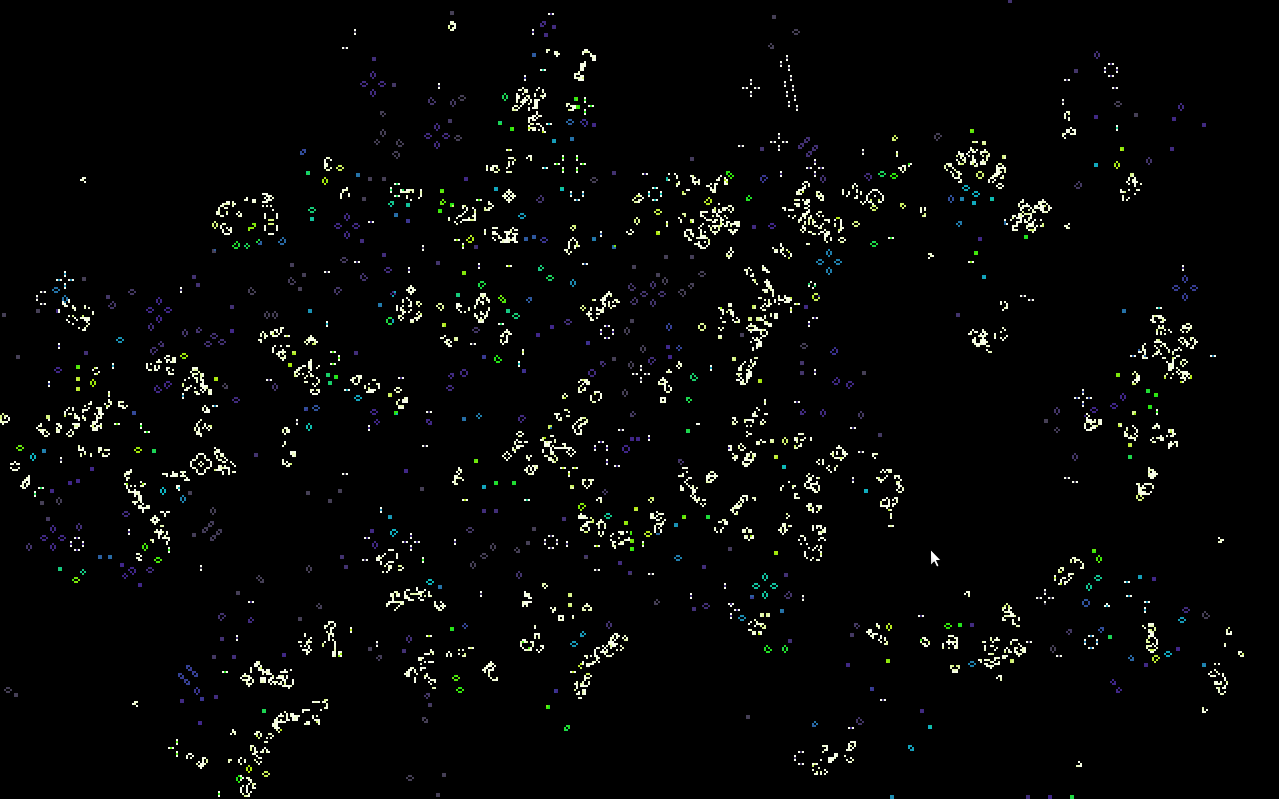
\includegraphics[width=18cm,angle=270]{life.png}
	\caption{Hra s náhodnou počáteční konfigurací}
\end{figure}

\end{document}
